\documentclass[14pt,usenames,dvipsnames]{beamer}
\usepackage[utf8]{inputenc}
\usefonttheme{structurebold}
\usepackage{cabin}
\usepackage[absolute,overlay,showboxes]{textpos}
\usepackage{multimedia}
\usepackage{ragged2e}
\usepackage{appendixnumberbeamer}


\usetheme{Madrid}
\usecolortheme{default}

\setbeamertemplate{itemize items}[triangle]
%\setbeamercolor{section number projected}{bg=blue,fg=white}
\setbeamertemplate{section in toc}[ball]
\setbeamertemplate{subsection in toc}[triangle]
\setbeamertemplate{section in toc}{\inserttocsectionnumber.~\inserttocsection}
\setbeamertemplate{subsection in toc}{\hspace{1.2 em}\textcolor{structure.fg}{$\blacktriangleright$}\inserttocsubsection \\}
%\setbeamertemplate{section in toc}{\hspace*{1em}\inserttocsection}
%\setbeamertemplate{subsection in toc}{\hspace*{2em}\inserttocsubsection}
\setlength{\leftmargini}{10pt}
\setbeamertemplate{blocks}[rounded][shadow=false]


%------------------------------------------------------------
%This block of code defines the information to appear in the
%Title page
\title[About Beamer] %optional
{A Secure Password Wallet based on the SEcube™ framework}


\author % (optional)
{Walter Gallego Gómez}

\institute[VFU] % (optional)
{
 Department of control and computer engineering\\
Politecnico di Torino
}

\date[VLC 2014] % (optional)
{July 23, 2018}

\titlegraphic{   \includegraphics[width=2cm]{logopolito}
   }



%\logo{\includegraphics[height=1.5cm]{logo-polito}}

%End of title page configuration block
%------------------------------------------------------------



%------------------------------------------------------------
%The next block of commands puts the table of contents at the 
%beginning of each section and highlights the current section:

\AtBeginSection[]
{
{\setbeamertemplate{footline}{} 
\begin{frame}[noframenumbering]
    \frametitle{Outline}
    \tableofcontents[currentsection]
  \end{frame}
}
}
%------------------------------------------------------------


\begin{document}




%gets rid of bottom navigation bar and adds numbers in custom size and color
\setbeamerfont{page number in head/foot}{size=\scriptsize}
\setbeamercolor{page number in head/foot}{fg=NavyBlue}
\setbeamertemplate{footline}[frame number]{}

%gets rid of navigation symbols
\setbeamertemplate{navigation symbols}{}

{\setbeamertemplate{footline}{} 
\begin{frame}[noframenumbering]
\titlepage
\end{frame}
} %this removes the footline from title page


\begin{frame}
\frametitle{Motivation}
The need for a hardware-based password manager is justified answering these three questions:


\begin{block}<2->{Are passwords still relevant?}
\onslide<3-> {Yes, they are the dominant form of authentication.}
\end{block}

\begin{block}<4->{Why should people use password managers?}
\onslide<5-> {So they can use unique strong passwords.}
\end{block}

\begin{block}<6->{Why are hardware-based approaches more reliable?}
\onslide<7-> {To authenticate, Master password + Device are required}
\end{block}

%\begin{itemize}
%    \item<1-> Are passwords still relevant?
%    
%    \onslide<2> {Yes, dominant form of authentication}
%
%    \item<3-> Why should people use password managers?
%    
%   \onslide<4> {Yes, dominant form of authentication}
%
%    \item<5-> Why are hardware-based approaches more reliable?
%
%   \onslide<6> {Yes, dominant form of authentication}
%\end{itemize}

\end{frame}



%---------------------------------------------------------
%This block of code is for the table of contents after
%the title page
\begin{frame}
\frametitle{Outline}
\tableofcontents
\end{frame}
%---------------------------------------------------------


\section{Introduction}



\begin{frame}
\frametitle{Introduction}
This work regards the implementation as a desktop application that exploits the capabilities of the SEcube™ (Secure Environment cube) hardware and software framework to store and protect passwords.

\vspace{10pt}
The desktop application, named \textbf{SEcubeWallet}, was written in C/C++and Qt, and it interacts with a SEcube™ device, requesting services like authentication and encryption/decryption of data.
\end{frame}



\section{Technologies used}

\subsection{Software libraries}
%---------------------------------------------------------
%Highlighting text
\begin{frame}
\frametitle{Software Libraries}

The following open source libraries were used:
{
\setbeamercolor{block title}{use=structure,bg=MidnightBlue,      fg=white}
\setbeamercolor{block body} {use=structure,bg=MidnightBlue!10!white, fg=black,}

\begin{block}<2->{Qt: GUI and wrappers}
\onslide<3-> {C++ library, cross-platform, elegant design}
\end{block}

\begin{block}<4->{SQLite: DataBase management}
\onslide<5-> {Self-contained, written in C, Transactional}
\end{block}

\begin{block}<6->{PwGen: Password generator}
\onslide<7-> {Configurable, random or readable}
\end{block}

\begin{block}<8->{zxcvbn: Password strength estimator}
\onslide<9-> {Dictionaries, keyboard patterns, sequences, years}
\end{block}
}
\end{frame}

% ----------------------------------

\subsection{The SEcube™ Framework}

\begin{frame}
  \frametitle{The SEcube™ Open Security Platform}
  \vspace{-0.3cm}

  \begin{columns}
    \column{0.5\textwidth}
	    \minipage[t][\textheight][t]{\columnwidth}
	    {\setbeamertemplate{blocks}[rounded][shadow=false]
	    \setbeamercolor{block title}{use=structure,bg=PineGreen, fg=white}
	    \setbeamercolor{block body} {use=structure,bg=white,     fg=black}
	    
	    \begin{block}{Hardware}
	      {\fontsize{14pt}{14}\selectfont
				\setbeamertemplate{blocks}[rounded][shadow=false]
				\setbeamercolor{block body} {use=structure,bg=PineGreen!10!white, fg=black,}
				\setbeamercolor*{item}{fg=PineGreen}
				\vspace{-0.3cm}
				
				\begin{block}<2->{}
	  			{Developed by the Blu5 Group}
				\end{block}
				
				\vspace{-0.2cm}
		
				\begin{block}<3->{}
				{
					\textbf{Family}
					\begin{itemize}
						\item SEcube™ Chip
						\item SEcube™ DevKit
						\item USEcube™ Stick
					\end{itemize}
				}
				\end{block}
				
				\vspace{-0.2cm}
				
				\begin{block}<4->{}
				{
					\textbf{SEcube™ Chip}
					\begin{itemize}
						\item \textbf{\color{PineGreen} MCU:} STM32F4 (STM)
						\item \textbf{\color{PineGreen} FPGA:} MachXO2-7000 (Lattice)
						\item \textbf{\color{PineGreen} Smart Card:} SLJ52G (infineon)
					\end{itemize}
				}
				\end{block}
			  }
	    \end{block}
	    }
	  \endminipage
  \column{0.5\textwidth}
	  \minipage[t][\textheight][t]{\columnwidth}
	  {\setbeamertemplate{blocks}[rounded][shadow=false]
	  \setbeamercolor{block title}{use=structure,bg=Red!90!Black,fg=white}
	  \setbeamercolor{block body} {use=structure,bg=white,       fg=black}
  	\begin{block}{Software}
	      {\fontsize{14pt}{14}\selectfont
				\setbeamertemplate{blocks}[rounded][shadow=false]
				\setbeamercolor{block body} {use=structure,bg=Red!10!white, fg=black,}
				\setbeamercolor*{item}{fg=Red}
				\vspace{-0.3cm}
				
				\begin{block}<5->{}
  			  Developed by European research institutions. \\
  			  Written in C using the Eclipse IDE. 
	  			
				\end{block}
								\vspace{-0.2cm}

				\begin{block}<6->{}
				   \textbf{Firmware:}
				   Developers can customize the firmware to their needs, and load the updated version to the SEcube™ chip.
				\end{block}				
								\vspace{-0.2cm}

				\begin{block}<7>{}
				  \textbf{Host libraries:}
           Allow to experience the platform as a high-security black box.
				\end{block}
				
		}		
	  \end{block}
	  }
	  \endminipage      
  
  \end{columns}
\end{frame}

\begin{frame}
\frametitle{SEcube™ APIs hierarchy}
\setlength{\TPboxrulesize}{1pt}
%\TPMargin{0pt}
\textblockrulecolour{red!70!black}
%\textblockrulecolour{white}
\textblockcolour{red!10!white}
\setbeamercolor*{item}{fg=red!70!black}

\begin{center}
\includegraphics<1>[width=\textwidth,height=0.8\textheight,keepaspectratio]{levelsHW}
\includegraphics<2>[width=\textwidth,height=0.8\textheight,keepaspectratio]{levelsL0}
\includegraphics<3>[width=\textwidth,height=0.8\textheight,keepaspectratio]{levelsL1}
\includegraphics<4>[width=\textwidth,height=0.8\textheight,keepaspectratio]{levelsL2}
\includegraphics<5>[width=\textwidth,height=0.8\textheight,keepaspectratio]{levels}
\end{center}

\only<2->{
\setlength{\leftmargini}{16pt}
\footnotesize \color{black} 
 \begin{textblock}{5}(10,2.2)
  \only<2>{
	  \begin{itemize}
	  \setlength\itemsep{-3pt}
	   \item Discover Devices 
	   \item Open Connection 
	   \item TX RX Data 
	   \item Close Connection
	  \end{itemize}
  }
  \only<3>{
	  \begin{itemize}
	  \setlength\itemsep{-3pt}
%	  \item Login
%	  \item Encrypt Data
%	  \item Decrypt Data
%	  \item Digest (Sign) Data 	  
    \item Pin and Keys init.
    \item Login \& Logout
    \item Information retrieval
    \item Encryption/decryption
    \item Digest (Sign)
    \item Key management 	  
	  \end{itemize}
  }
  \only<4>{
	  \begin{itemize}
	  \setlength\itemsep{-3pt}
	  \item SEfile
	  \item secureSQLite
	  \item SElink
	  \end{itemize}
   }  
  
  \only<5>{
    \vspace{5pt}
    \hspace{5pt}\textbf{Applications}
  	\begin{itemize}
	  \setlength\itemsep{-3pt}
	  \item secureSQLiteBrowser
	  \item \textbf{\color{red!70!black} SEcubeWallet}
	  \end{itemize}
	  }
 \end{textblock}
}

\end{frame}

%---------------------------------------------------------------

\section{Design and implementation}

\subsection{General Architecture}

\begin{frame}
	\only<1>{\frametitle{SEcubeWallet Application}}
	\only<2>{\frametitle{Open device and authenticate}}
	\only<3>{\frametitle{Create In-memory Wallet}}
	\only<4>{\frametitle{Generate Password/Passphrase}}
	\only<5>{\frametitle{Evaluate Strength}}
	\only<6>{\frametitle{Encrypt and Save Wallet to disk}}
	\only<7>{\frametitle{General Architecture}}
	\begin{center}
	\includegraphics<1>[width=\textwidth,height=0.85\textheight,keepaspectratio]{BasicDesignOnly}
	\includegraphics<2>[width=\textwidth,height=0.85\textheight,keepaspectratio]{BasicDesignLog}
	\includegraphics<3>[width=\textwidth,height=0.85\textheight,keepaspectratio]{BasicDesignInMem}
	\includegraphics<4>[width=\textwidth,height=0.85\textheight,keepaspectratio]{BasicDesignGen}
	\includegraphics<5>[width=\textwidth,height=0.85\textheight,keepaspectratio]{BasicDesignZ}
	\includegraphics<6>[width=\textwidth,height=0.85\textheight,keepaspectratio]{BasicDesignDisk}
	\includegraphics<7>[width=\textwidth,height=0.85\textheight,keepaspectratio]{BasicDesign}
	
	\end{center}
\end{frame}

\subsection{Basics of Operation}

\begin{frame}
	\frametitle{Basics of Operation}
{\fontsize{13pt}{14}\selectfont	
	\begin{itemize}
	\setlength\itemsep{15pt}
	 \item<2-> At factory initialization, an admin/developer writes to the SEcube™ flash memory:
	   \begin{itemize}
	   	
	     \item<2-> {\fontsize{12pt}{14}\selectfont Admin pin}
	     \item<2-> {\fontsize{12pt}{14}\selectfont User pin}
	     \item<2-> {\fontsize{12pt}{14}\selectfont User Keys}
	   \end{itemize}
	 \item<3-> User logins with its pin and a challenge-based authentication.
	 \item<4-> User chooses which of the keys to use to encrypt/decrypt.	  
	\end{itemize}
	
\begin{alertblock}<5->{The data (passwords) can only be accessed if:}
 \begin{itemize}
       \setlength\itemsep{0pt}
	     \item<2-> SEcube™ device is connected
	     \item<2-> Login pin is the correct one
	     \item<2-> Key inside the device is the correct one.
	   \end{itemize}
\end{alertblock}	
}	
\end{frame}

\begin{frame}
	\frametitle{In-Memory and In-Disk DBs}
  \begin{itemize}
  \setlength\itemsep{10pt}
    \item<2-> \textbf{New Wallet:} An In-memory SQLite DB is created.
    \item<3-> \textbf{Save Wallet:} An In-disk encrypted secureSQLite DB is created and populated with the In-memory DB contents
    \item<4-> \textbf{Open Wallet:} The selected In-disk DB is decrypted and its contents are dumped into an In-memory DB
    \item<5-> \textbf{Delete Wallet:} Both the In-memory DB and the In-disk encrypted file are deleted.
  \end{itemize}
\end{frame}

\subsection{Implementation details}

\begin{frame}
	\frametitle{Windows and display elements}

  \begin{itemize}
    \setlength\itemsep{10pt}
    \item<2-> Main Window
      \begin{itemize}
		    \item \textbf{\color{NavyBlue} Table View} for displaying the wallet entries
		    \item \textbf{\color{NavyBlue} Filters} So the user can search in each of the table's columns.
		    \item \textbf{\color{NavyBlue} Tool Bars} for Wallets, Tables and Entries.
		    \item \textbf{\color{NavyBlue} Menu Bar} with all the actions.
		    \item \textbf{\color{NavyBlue} Status Bar} used to display messages and the wallet's name
      \end{itemize}
      
     \item<3-> Preference Window
       \begin{itemize}
	       \item Password Generators Configuration.
	       \item zxcvbn Configuration.
	     \end{itemize}
     \item<4-> Help Window
     \item<5-> Environment Window
	 \end{itemize}
\end{frame}



\begin{frame}
	\frametitle{Data Display: Model/View architecture}

  \begin{columns}
   \column{0.4\textwidth}
      \includegraphics<2->[width=1\columnwidth]{modelview.png}
    \column{0.6\textwidth}	
			\begin{itemize}
			\setlength\itemsep{10pt}
			
			\item<3-> \textbf{Data:} Entries in a table from the In-memory DB.
			\item<4-> \textbf{Model}: Wrapper for handling SQLite DBs easily. 
			\item<5-> \textbf{Proxy Model}: Custom filtering for each column.
			\item<6-> \textbf{View}: Data is displayed as a table.
			\item<7-> \textbf{Delegate}: Used to Show/Hide the passwords.
			\end{itemize}	
	\end{columns}
\end{frame}

\begin{frame}
  \frametitle{SW Libraries}

	  \begin{block}<2->{zxcvbn: Password strength estimator}
		\begin{itemize}
		\setlength\itemsep{0pt}
			\item C/C++ open sources.
			\item Included in the project as a \textbf{\color{NavyBlue} Dynamic Library}
		\end{itemize}
	\end{block}


	\begin{block}<3->{PwGen: Pronounceable Passwords Generator}
    The sources were modified (simplified) and included in the application.
  \end{block}


	\begin{block}<4->{PassPhrase Generator}
		\begin{itemize}
				\setlength\itemsep{0pt}
		  \item Implemented as a C++/Qt function.
		  \item Works by extracting Random words out of dictionary files (plain text).
		\end{itemize}
  \end{block}
\end{frame}

\begin{frame}
	\frametitle{Other functionalities}
  \begin{itemize}
  	\setlength\itemsep{25pt}
    \item<2-> \textbf{Search for expired passwords} \\
    Using date's column custom filter
    \item<3-> \textbf{Launch entry's domain} \\
    In default OS web browser
    \item<4-> \textbf{l33t converter} \\
    From {\color{NavyBlue} PenicuikCiting} to {\color{NavyBlue} 9en1cu1kC1t1ng}.

  \end{itemize}  	
	
\end{frame}



%-------------------------------------------

\section{Demos}

\begin{frame}
\frametitle{Login and Open a Wallet}
\begin{center}
\makebox[0pt]{
\movie[
  width=1.08\textwidth,
  height=0.57\textwidth, 
  showcontrols,
  poster
] 
{
\includegraphics[width=1.08\textwidth]{playbutton.pdf}}{loginOpen.mkv}
}
\end{center}
\end{frame}

%-------------------------------------

\begin{frame}
	\frametitle{Generate and evaluate password}
	\begin{center}
	\vspace{-0.4cm}
	\makebox[0pt]{ %no left margin
		\movie[
		  width=1.03\textwidth,
		  height=0.72\textwidth, 
		  showcontrols,
		  poster
		] 
		{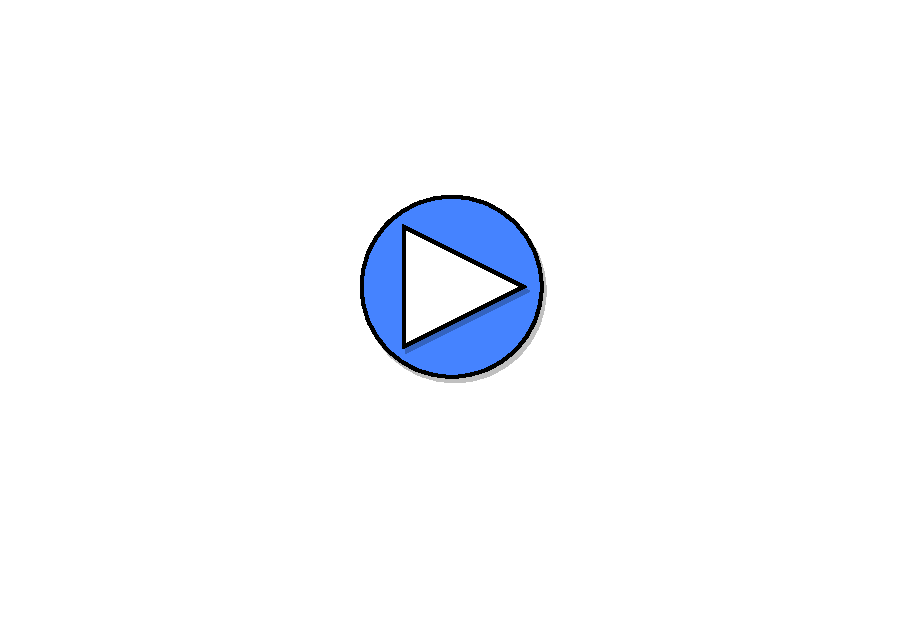
\includegraphics[width=1.03\textwidth]{playbutton2.pdf}}{add.mkv}
	}
	\end{center}
\end{frame}

\section{Conclusions}
\begin{frame}
	\frametitle{Conclusions}
	\begin{itemize}
		\setlength\itemsep{10pt}
		\item<1-> The SEcube™ is perfect for this type of application as it offers both reliability and simplicity to use.
		\item<2-> In any password manager it is important to suggest random passwords and to check their strength
		\item<3-> All the used libraries in this project are open source, proving it is possible to achieve a high level of security with the use of open software and hardware tools. 
		\item<4-> The developed application still lacks some features in order to be considered a truly commercial product.
	
	\end{itemize}
\end{frame}

\section{Future Work}
\begin{frame}
	\frametitle{Future Work}
	{
	\setbeamercolor{block title}{use=structure,bg=MidnightBlue,          fg=white}
	\setbeamercolor{block body} {use=structure,bg=MidnightBlue!10!white, fg=black,}
  \fontsize{14pt}{14}\selectfont

	
  \vspace{-0.3cm}	
	  
	\begin{block}<2->{Web Browse Integration}
  \setbeamercolor*{item}{fg=MidnightBlue}
		\begin{itemize}
		  \item Port the entire Application to a web browser complement.
			\item Web browser complement that "talks" with the SEcubeWallet
			\item Use keyboard emulation to Auto Fill forms
		\end{itemize}
	\end{block}

	\vspace{-0.1cm}	

	\begin{block}<3->{More than static passwords}
	\setbeamercolor*{item}{fg=MidnightBlue}
		\begin{itemize}
			\item One Time Passwords
			\item FIDO U2F
		\end{itemize}
	\end{block}
	
	\vspace{-0.1cm}	
	
	\begin{block}<4->{Android}
	\setbeamercolor*{item}{fg=MidnightBlue}
		\begin{itemize}
			\item Use a SEcube™ phone device
			\item Port SEcube™ host-side libraries to android
			\item Port Qt application to android
		\end{itemize}
	\end{block}	
	}
	
\end{frame}

%%%%%%%%%% backup slides %%%%%%%%%%

\appendix

\section*{SEfile}
\begin{frame}
	\frametitle{SEfile}
	
	A secured file has the structure shown in figure. The data is divided in sectors, and each of them is encrypted and signed. The first sector (header) contains metadata.
	
	When a portion of the file wants to be read or written, it is not necessary to process the whole file. Only the required sectors are manipulated.
	
	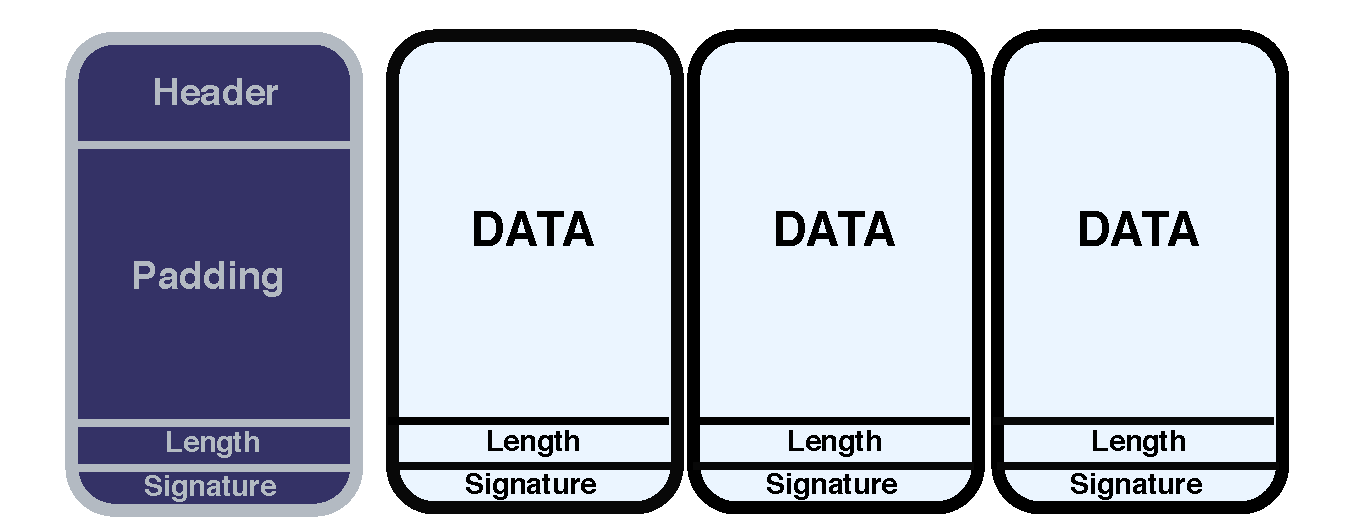
\includegraphics[width=1\columnwidth]{secfile}	

\end{frame}

\section*{Algorithms}

\begin{frame}
	\frametitle{Algorithms}
	
	\textbf{Encryption}: Advanced Encryption Standard (AES), established by the U.S. National Institute of Standards and Technology (NIST). For each data sector {\color{NavyBlue} AES-256-CTR} is used, while the header sector is encrypted using {\color{NavyBlue}AES-256-ECB}.
	
	\vspace{7pt}
	
	\textbf{Authentication} Each sector, including the header, is signed using {\color{NavyBlue} SHA-256-HMAC}, meaning that the signature depends on both the data contained in the sector itself and on a chosen encryption key. 
	
	\vspace{7pt}
	
	To use two different keys to encrypt data and to digest authentication. SEfile leverages on the pbkdf2()
\end{frame}

\section*{secureSQLite}

\begin{frame}
	\frametitle{secureSQLite}
	
	Based on the {\color{NavyBlue} SQLite} and {\color{NavyBlue} SEfile}, this API allows the user to create SEcube™ secured data bases.
	
	\vspace{7pt}
	
  The SQLite system has been modified to use a wrapper based on SEfile, rather than using directly the OS calls. The development is based on a template for making a custom {\color{NavyBlue} VFS} interface distributed along with SQLite.

\vspace{7pt}

Every database created with secureSQLite is cyphered and signed, thus making it impossible to read the database contents without the SEcube™.
\end{frame}

\section*{DevBoard}

\begin{frame}
	\frametitle{Development Board}
	
	\begin{columns}
    \column{0.5\textwidth}
			\begin{description}
				\setlength\itemsep{-3pt}
				\fontsize{11pt}{14}\selectfont
				\item  [J1000] USB 2.0 to UART 
				\item [J2000]  Ethernet 10/100 
				\item [J4000]  FPGA and CPU GPIOs
				\item [J4001]  JTAG
				\item [J4002]  microSD card 
			\end{description}    
    
      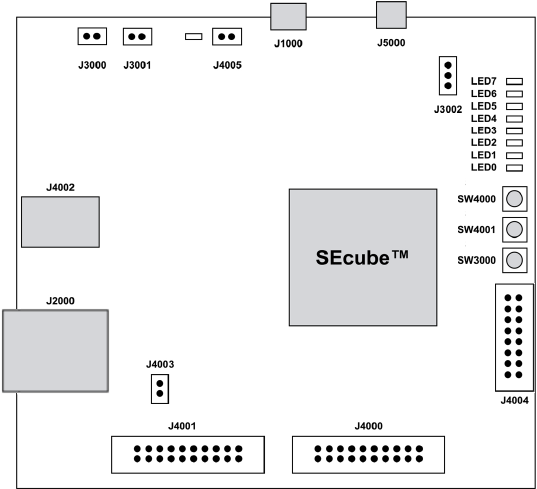
\includegraphics[width=\columnwidth]{devboard_sch}
    \column{0.5\textwidth}
			\begin{description}
			\fontsize{11pt}{14}\selectfont
				\setlength\itemsep{-3pt}
				\item [J4004]  FPGA and CPU GPIOs
				\item [J5000]  USB 2.0 High Speed 
				\item [LEDx]   Leds 
				\item [SWx00y]  Switches 
			\end{description}       
    
      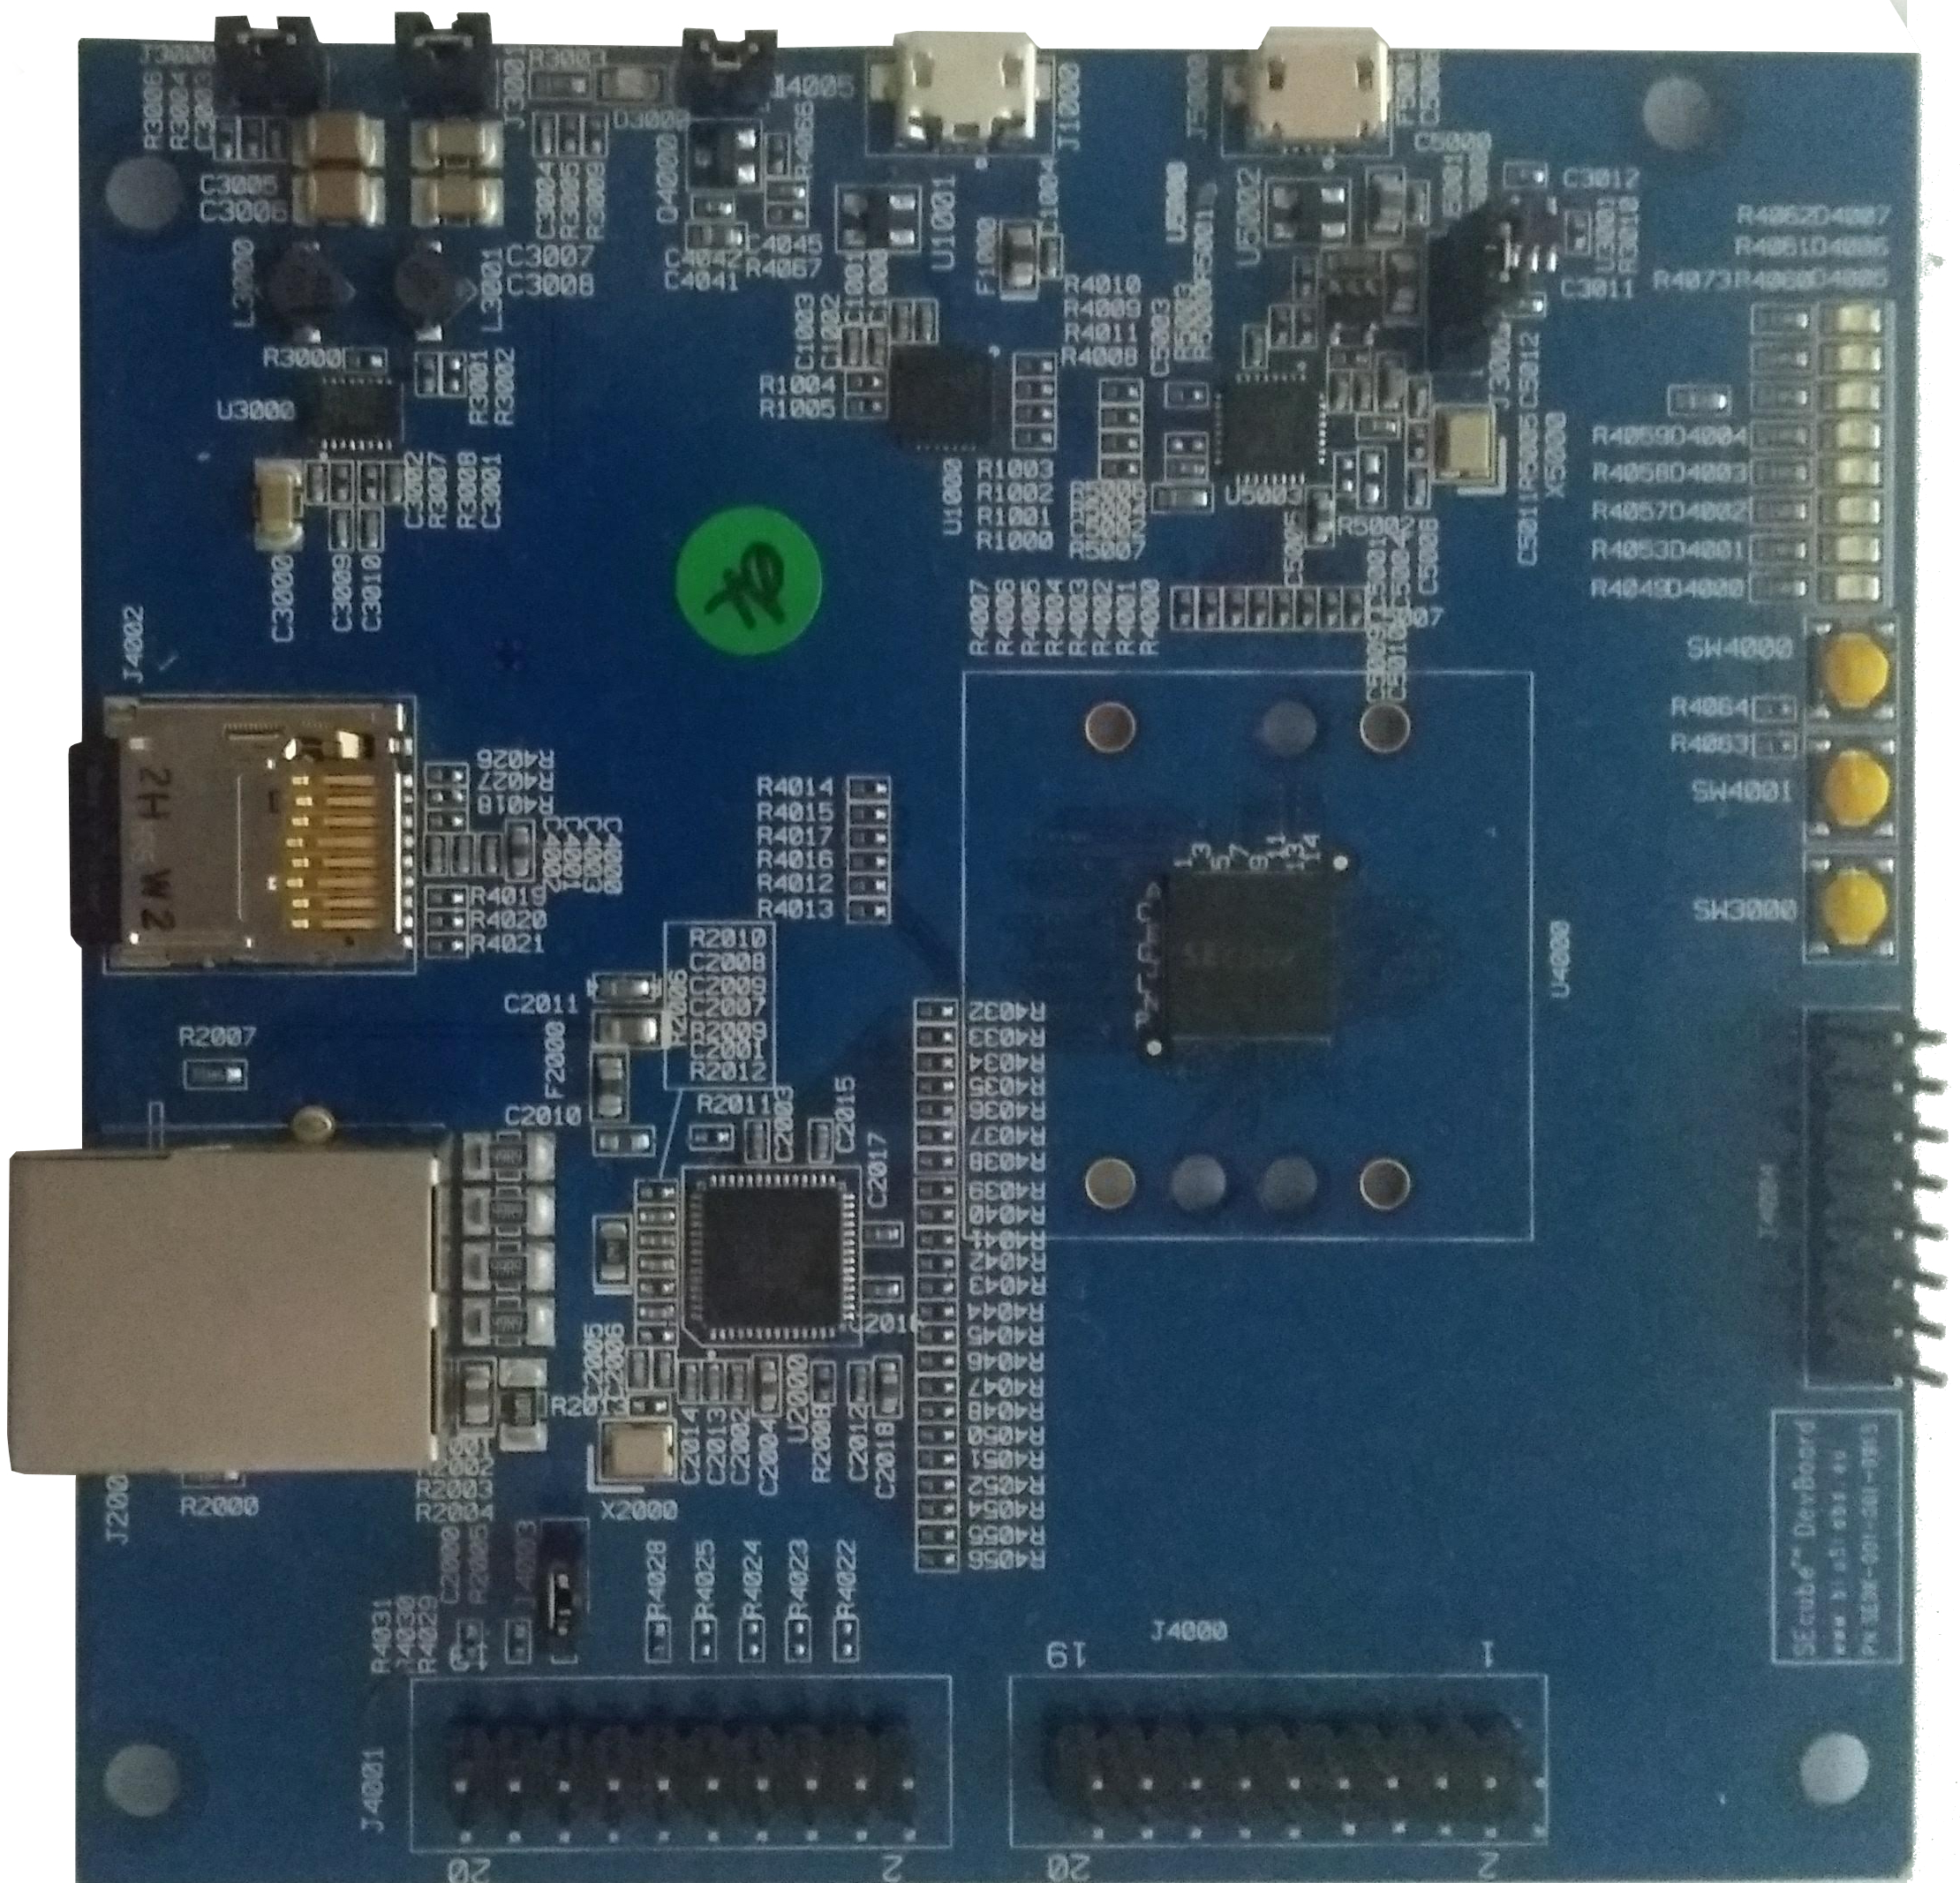
\includegraphics[width=\columnwidth]{devboard}
  \end{columns}
\end{frame}

\begin{frame}
	\frametitle{JTAG Connections}
	
To program and debug the chip, we use an \textbf{{\color{NavyBlue}ST-Link/V2}} which communicates with the MCU using the JTAG/SWD connection in the DevKit board.

  \begin{columns}
    \column{0.5\textwidth}  
      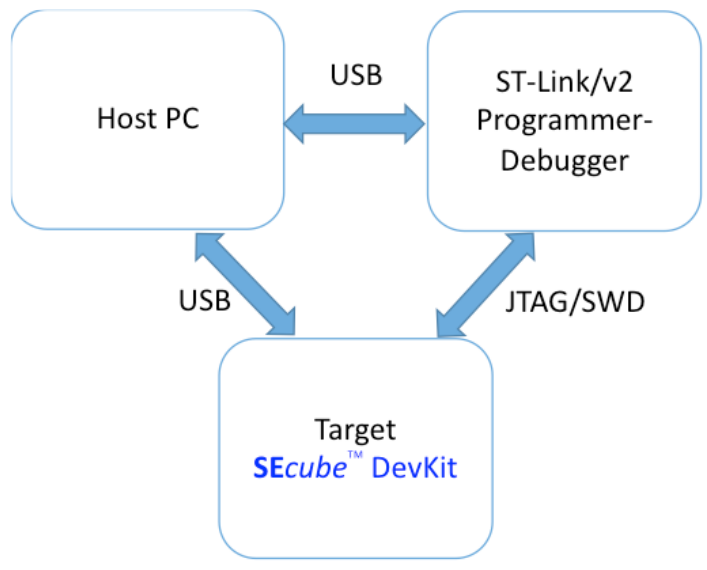
\includegraphics[width=\textwidth]{conSche}
    \column{0.5\textwidth}  
      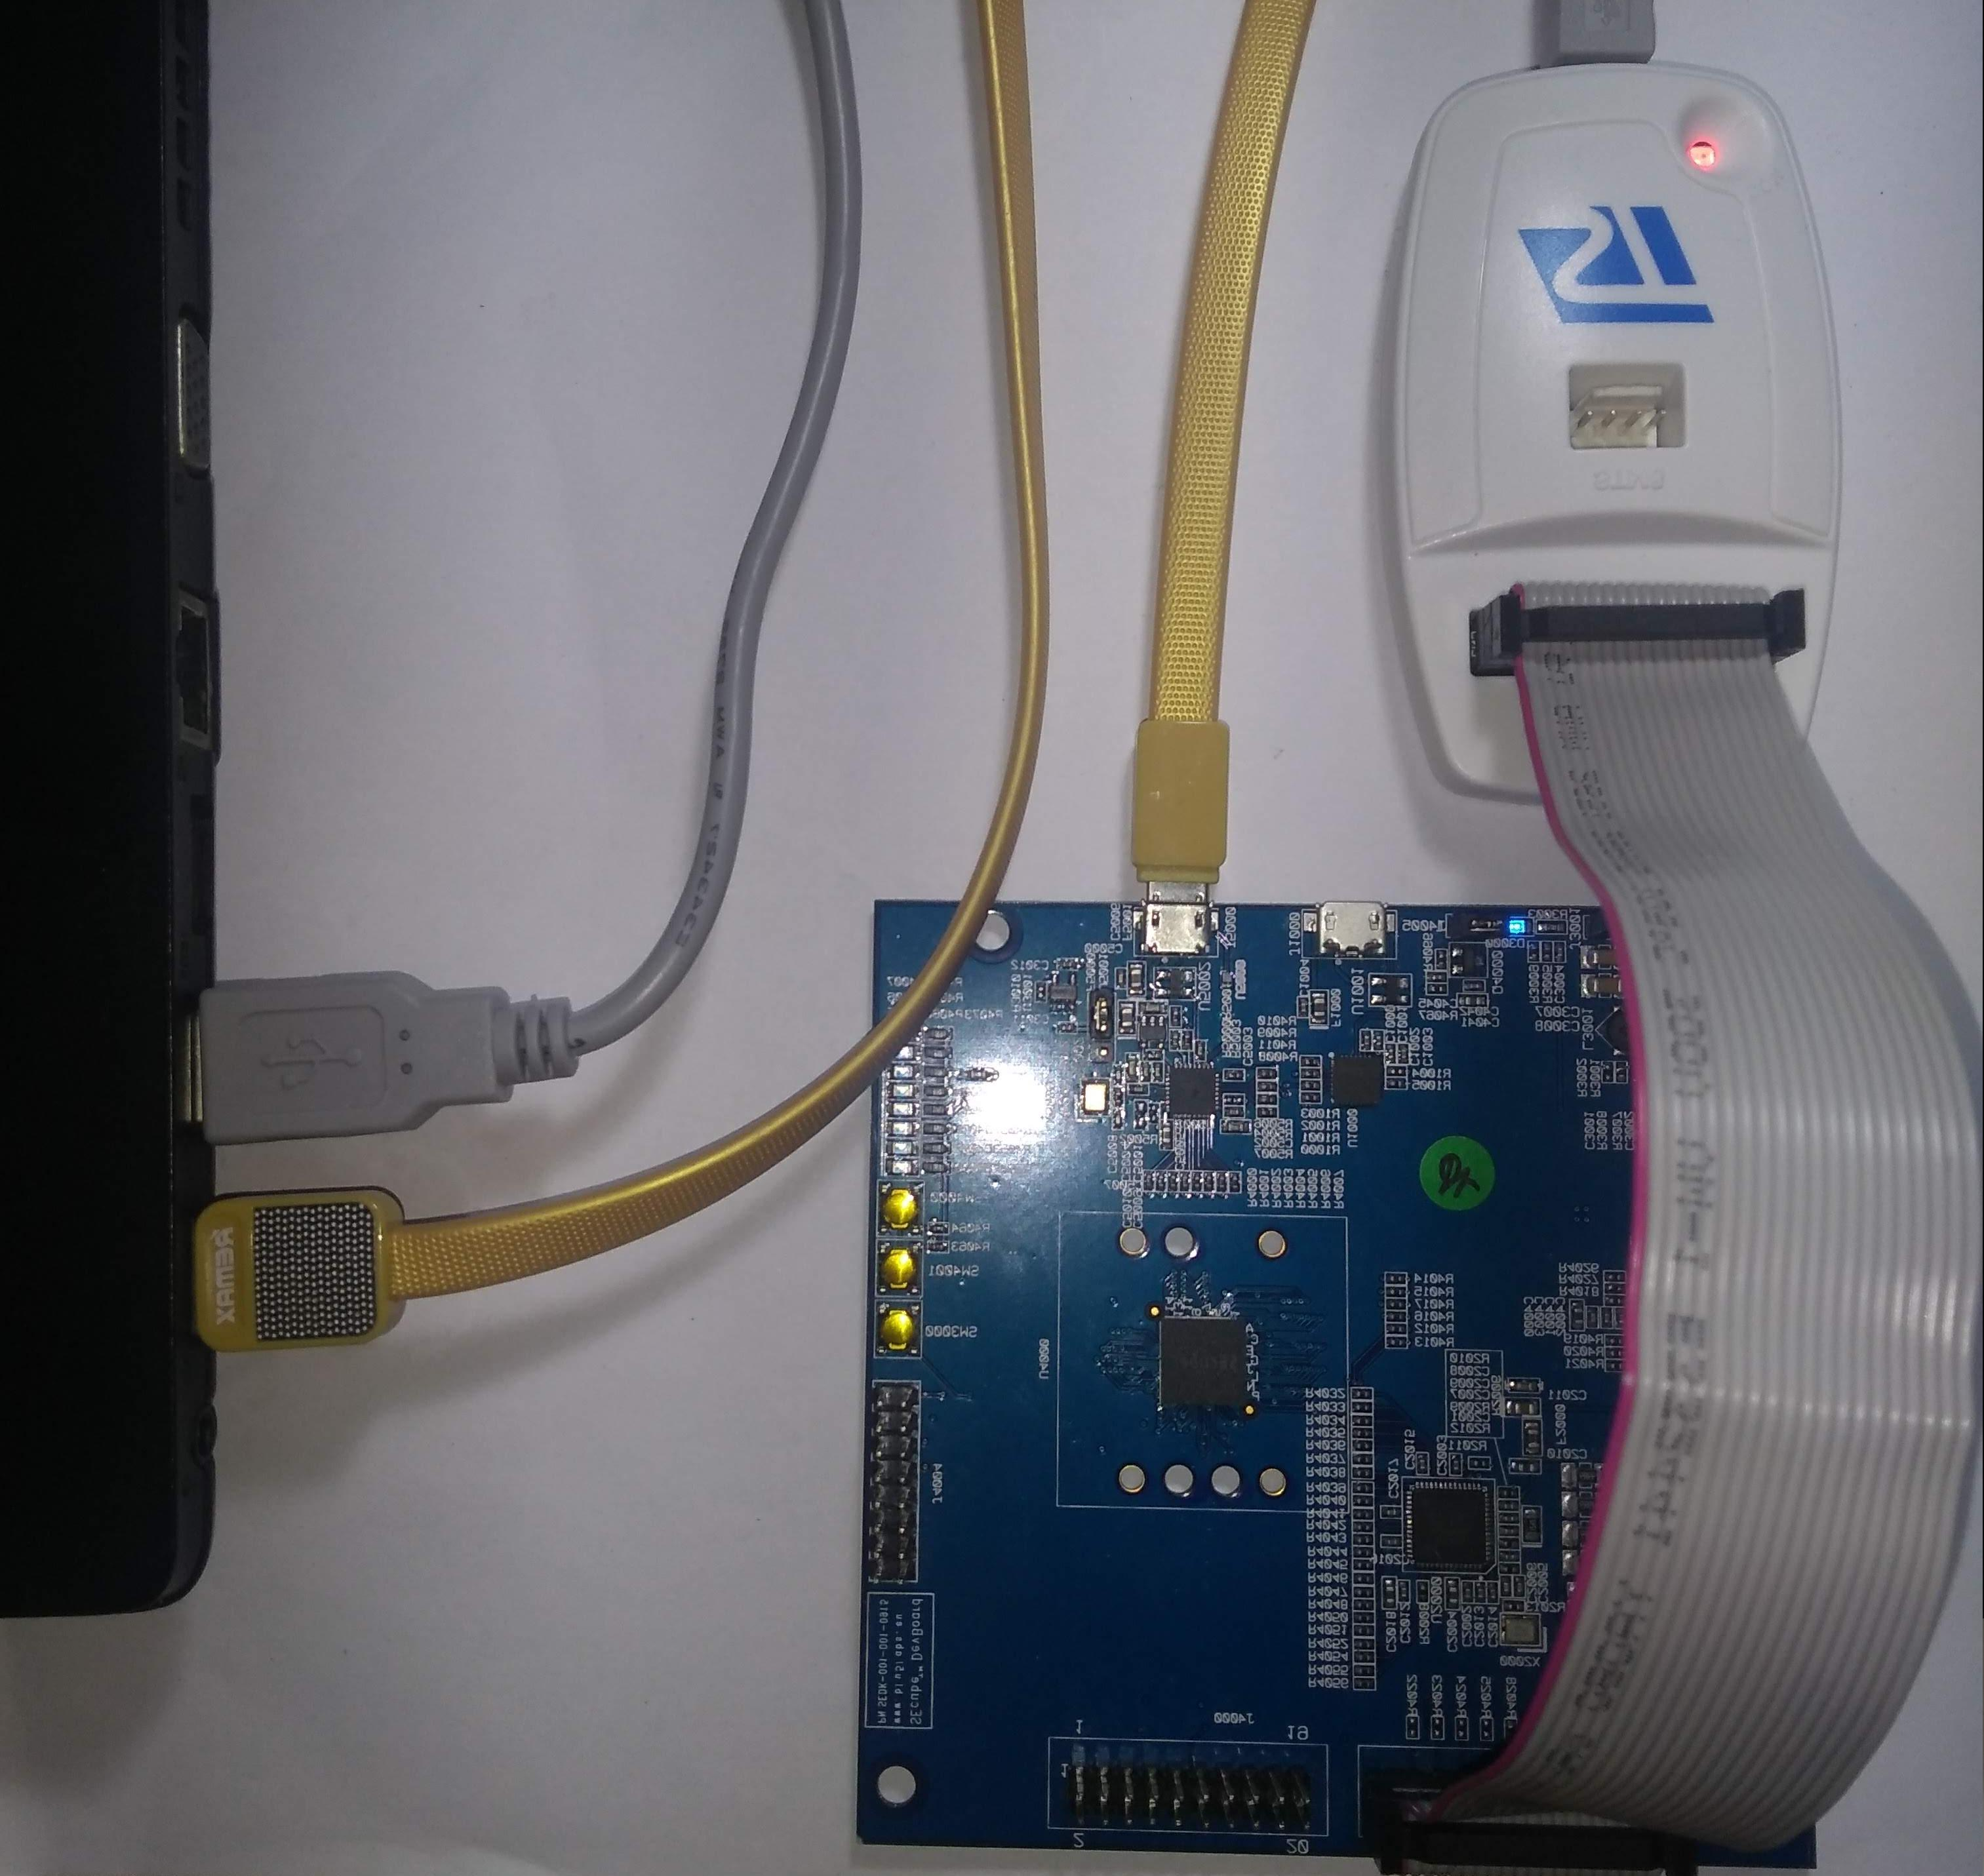
\includegraphics[width=\textwidth]{conReal2}
  \end{columns}
\end{frame}

\section*{USEcube}

\begin{frame}
	\frametitle{The USEcube™ Stick}
  \begin{itemize}
      \setlength\itemsep{-1pt}  
		  \fontsize{12pt}{14}\selectfont
				
				\item {\color{NavyBlue} SEcube™ chip + USB 2.0 High-Speed + SDcard socket.}
				\item Compatible with any Operating System, and no need for drivers.
				\item Separation of encrypted data from the encryptor/decryptor. 				
				\item microSD can be changed to adjust size and speed.
				\item Dust and water-resistant
				\item No JTAG interface. To inject firmware, secure bootloader.
	  \end{itemize}
	
 	\begin{columns}
    \column{0.5\textwidth}
      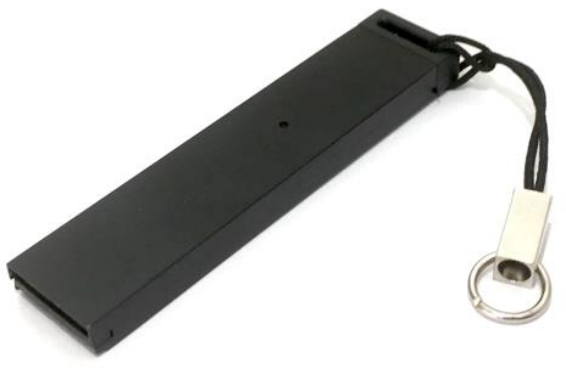
\includegraphics[width=\columnwidth]{usb.png}
    \column{0.5\textwidth}
      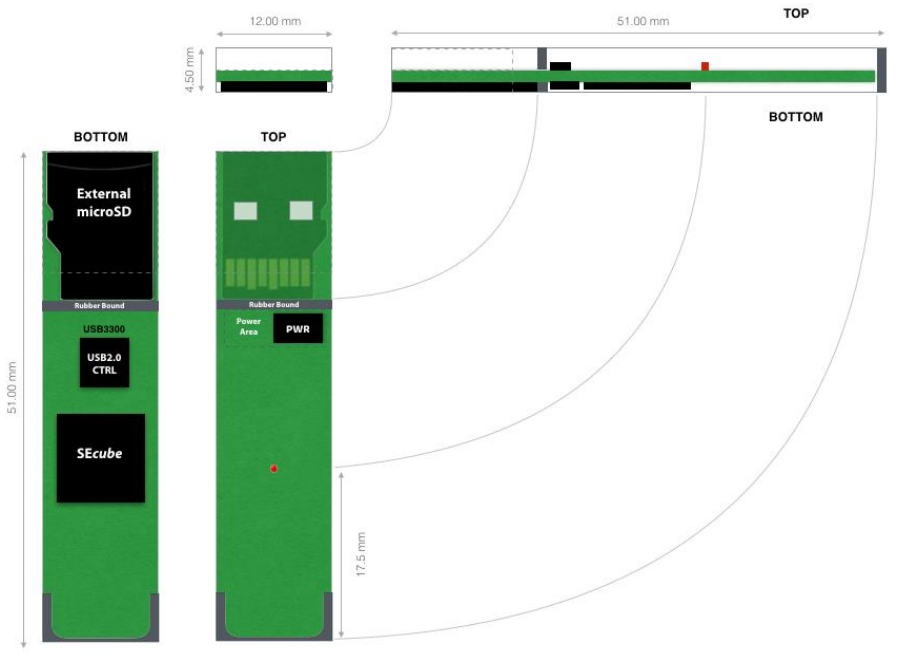
\includegraphics[width=\columnwidth]{usb_sch.png}
   \end{columns}
\end{frame}

\section*{YubiKey}

\begin{frame}
	\frametitle{YubiKey}
	
  {\fontsize{11pt}{14}\selectfont
	Family of hardware authentication devices developed by Yubico 
	Unfortunately, not open source.
	
	Supports Google Accounts, Facebook Accounts, GitHub, Dropbox
  }
  
  \begin{columns}
  \column{0.5\textwidth}
		\begin{itemize}
		\setlength\itemsep{-3pt}
	  \fontsize{11pt}{14}\selectfont	
			\item Static Passwords
			\item Yubico One-Time Password (OTP)
			\item OATH – HOTP (EVENT)
			\item OATH – TOTP (TIME)
	  \end{itemize} 
	  
  \column{0.5\textwidth}	  
  \begin{itemize}
	  \setlength\itemsep{-3pt}
	  \fontsize{11pt}{14}\selectfont	
			\item Challenge and Response (HMAC-SHA1, Yubico OTP)
			\item PIV-Compatible Smart Card: 	
			\item OpenPGP
			\item FIDO U2F
	  \end{itemize} 
	  
	\end{columns}
  \centering	
	  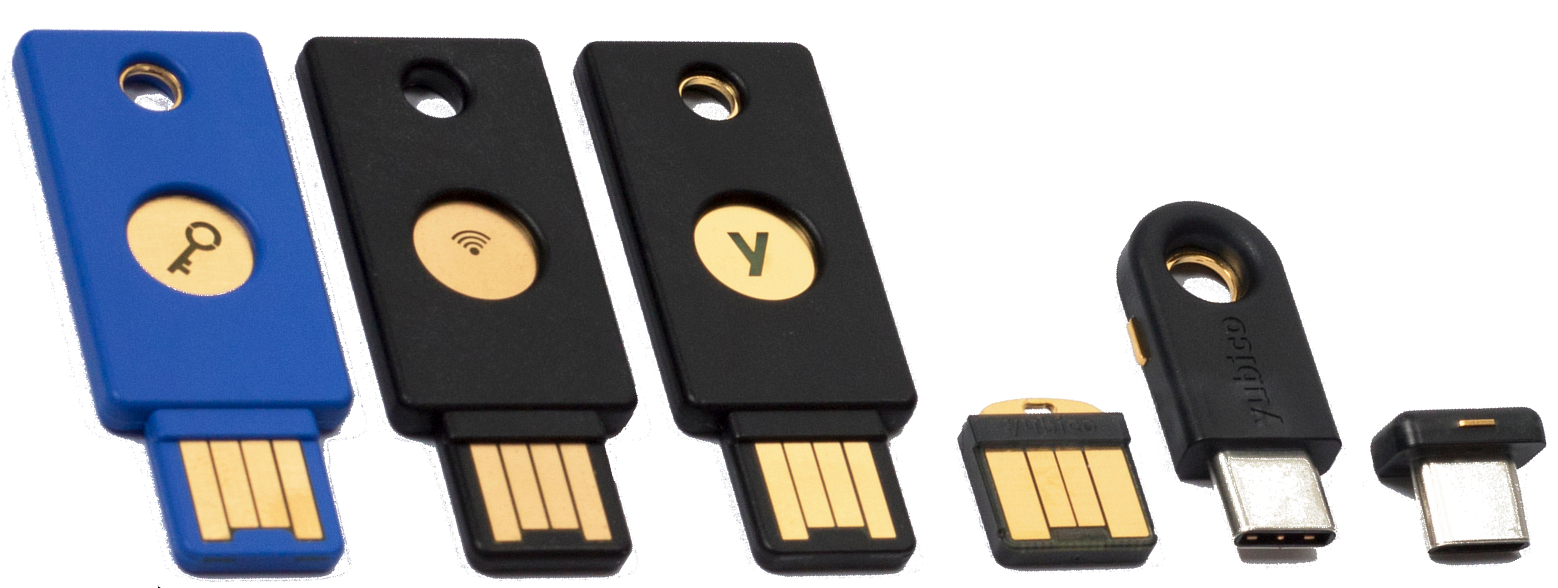
\includegraphics[width=0.8\columnwidth]{yubikeyfam.jpg}

	
\end{frame}

\section*{Mooltipass}

\begin{frame}
	\frametitle{Mooltipass: A Simple Offline Password Keeper}
  \fontsize{11pt}{14}\selectfont	
		\onslide<1->{The Mooltipass emulates a standard USB keyboard, 
		The Mooltipass has an internal flash in which the user encrypted credentials are stored, while a PIN-locked smartcard contains the AES-256bits key required for their decryption.
		Open software and open hardware, kickstarter campaign.}

 \begin{columns}
    \column{0.5\textwidth} 
			\begin{itemize}
				\setlength\itemsep{-3pt}
				\fontsize{11pt}{14}\selectfont	
				\item<2-> Plugin the Mooltipass, no driver required.
				\item<3-> Insert the smartcard and unlock it with the PIN
				\item<4-> If using the browser plugin, the Mooltipass asks permission to send the stored credentials, or asks you to save new ones
				\item<5-> If not using the browser plugin Mooltipass can type credentials like a keyboard.
			\end{itemize}

  \column{0.5\textwidth}
		\begin{itemize}
			\setlength\itemsep{-3pt}
			\fontsize{11pt}{14}\selectfont	
			
			\item<6-> \textbf{ST662ACD-TR:} Power
			\item<6-> \textbf{ATMEGA32U4:} MCU
			\item<6-> \textbf{AT88SC102:} Smart Card
			\item<6-> \textbf{AT45DB011D-SSH-T:} Flash
		\end{itemize}
		
		\includegraphics<6->[width=\columnwidth]{mooltipass.jpg}

  \end{columns}
\end{frame}

\section*{pwgen ex}

\begin{frame}
	\frametitle{PwGen Examples}

  \begin{columns}
	\column{0.5\textwidth}
    \texttt{-s}:	Random\\
    \texttt{-y}: Symbols\\
    \texttt{-v}: No vowels
  \column{0.5\textwidth}
    \texttt{-B}: No ambiguous\\
    \texttt{-A}: No capital\\
    \texttt{-0}: No numerals
	
	\end{columns}
	\begin{table}
		\begin{tabular}{c|c|c|r}
		\textbf{Password} & \textbf{Length} & \textbf{Options} & \textbf{Log Entropy}  \\ 
		\hline
		\hline
		
		\texttt{iesohGhai3}   & 10 & \texttt{-}    &  9.75 (Level 3)\\
		\texttt{ees0cooLo2}   & 10 & \texttt{-}    & 10.47 (Level 4)\\
		\texttt{dX042wKqlW}   & 10 & \texttt{-s}   & 17.86 (Level 4)\\
		\texttt{@!,Q*l5\}+H } & 10 & \texttt{-ys}  & 18.15 (Level 4)\\
		\texttt{TBw4)9}       &  6 & \texttt{-ys}  & 11.62 (Level 4)\\
		\texttt{B7t34Lck}     &  8 & \texttt{-v}   & 11.87 (Level 4)\\
		\texttt{nofosootei}   & 10 & \texttt{-BA0} &  6.50 (Level 2)\\
		\end{tabular}
  \end{table}

\end{frame}

\section*{passgen ex}

\begin{frame}
	\frametitle{PassPhrase Generator examples}
  	  \fontsize{11pt}{14}\selectfont	
	
	  \resizebox{\linewidth}{!}{% Resize table to fit within \linewidth horizontally
\begin{tabular}{c|c|c|c|r}
\textbf{PassPhrase} & \textbf{wor} & \textbf{len} & \textbf{uncom}  & \textbf{Log Entr} \\ 
\hline
\hline
		 {\color{NavyBlue}C}occhio & 1 & - & - & 4.27 (L1) \\ 
		 
		 {\color{NavyBlue}L}egitimately & 1 & 8 & - & 4.55 (L1) \\
     
     {\color{NavyBlue}W}oodhaven		& 1 & 8 & 30\% & 4.94 (L1) \\
     \hline    
     {\color{NavyBlue}S}horeline{\color{NavyBlue}C}ech & 2 & - & - & 9.18 (L3) \\
     
     {\color{NavyBlue}M}ongolia{\color{NavyBlue}S}impsons & 2 & 8 & -    & 7.30 (L2) \\
     {\color{NavyBlue}M}cinnis{\color{NavyBlue}P}haya     & 2 & - & 30\% & 9.14 (L3) \\

     {\color{NavyBlue}Z}ucchini{\color{NavyBlue}S}alamandra & 2 & 8 & 30\% & 9.19 (L3) \\
     {\color{NavyBlue}S}acchetti{\color{NavyBlue}V}igevano  & 2 & 8 & 30\% & 9.11 (L3) \\

     {\color{NavyBlue}D}rammaturgico{\color{NavyBlue}S}batacchiare  & 2 & 12 & - & 8.98 (L3) \\
     {\color{NavyBlue}M}alformations{\color{NavyBlue}A}strophysical & 2 & 12 & - & 9.60 (L3) \\
     \hline
     {\color{NavyBlue}L}atina{\color{NavyBlue}I}nterchange{\color{NavyBlue}F}bo & 3 & - & - & 13.5  (L4) \\
     {\color{NavyBlue}O}sa{\color{NavyBlue}A}yman{\color{NavyBlue}C}antinflas   & 3 & - & - & 12.98 (L4) \\
     {\color{NavyBlue}I}mmobile{\color{NavyBlue}C}w{\color{NavyBlue}S}ites      & 3 & - & - & 11.43 (L4) \\
     
     {\color{NavyBlue}R}immel{\color{NavyBlue}B}rag{\color{NavyBlue}F}aenza     & 3 & - & 30\% & 13.49 (L4) \\
     
     {\color{NavyBlue}R}eclining{\color{NavyBlue}C}anberra{\color{NavyBlue}E}cuadorian         & 3 & 8 &  -   & 13.69 (L4) \\
     
     {\color{NavyBlue}I}naspettato{\color{NavyBlue}R}othschilds{\color{NavyBlue}D}isconcerting & 3 & 8 & 30\% & 14.48 (L4) \\

\end{tabular}}	
\end{frame}

\section*{other contributions}

\begin{frame}
		\frametitle{Other contributions}
	Besides the application development, other results obtained during this work are:
	\begin{itemize}
	\setlength\itemsep{10pt}
		\item The implementation of an improved Login behaviour in the SEcube™ framework, that renders more usable SEcubeWallet and any other application that uses the SEcube™ authentication system.
		
		\item The discovery and fix of a bug in the SEfile library that did not allow to use the secureSQLite library in a FAT32 file system.
	\end{itemize}
		
\end{frame}

\section*{SEkey}

\begin{frame}
	\frametitle{SEkey: key management for SEcube™}
		  \fontsize{12pt}{14}\selectfont	

	
	SEkey is a new library currently under development by 	Mateus Françani as his master thesis work. The library will sit next to SEfile and SElink.
	
	\begin{columns}
	  \column{0.5\textwidth}
	    
	    Right now keys inside a SEcube™ chip can only be modified at factory reset. This is not very useful in a working environment, as the purpose of having multiple keys is to allow users to share information with selected people. 
	    
	\vspace{7pt}
	
	The job of the SEkey library will be to allow an admin to dynamically add and remove keys to SEcube™ devices.
	
	    \column{0.5\textwidth}  
	      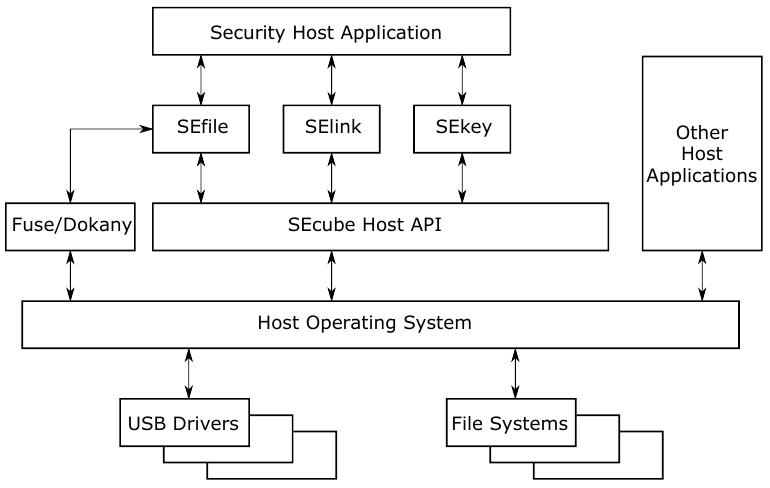
\includegraphics[width=\columnwidth]{sekey.png}
	  
	\end{columns}  

\end{frame}





\end{document}